% =============================================================================
%  Parallel BFS Poster: Linear Algebraic vs Graph-First on a Single GPU
%
%  Format : Matte stock, 40 in (W) x 30 in (H), landscape.
%  Layout : 25% Introduction | 50% Methods + Results | 25% Further Study
%  Engine : pdflatex (also lualatex / xelatex), tikzposter v2.x
%
%  Build  : pdflatex poster.tex   (run twice for cross-references)
%           or simply `make` -- see the included Makefile.
%
%  The poster emphasizes the completed single-GPU implementation and the
%  Perlmutter benchmark workflow used to collect final timing tables.
% =============================================================================

\documentclass[
    a0paper,
    margin=0.14in,
    innermargin=5mm,
    blockverticalspace=3mm,
    colspace=3mm,
    subcolspace=2mm,
    20pt,
]{tikzposter}

% --- Full-bleed style margins: maximal text width; bottom kept minimal but
%     not zero (trims on some print workflows start ~1/8 in from edge).
\geometry{paperwidth=40in, paperheight=30in,
          left=0.14in, right=0.14in, top=0.26in, bottom=0.14in}

\usepackage[utf8]{inputenc}
\usepackage[T1]{fontenc}
\usepackage{lmodern}
\usepackage{amsmath, amssymb}
\usepackage{booktabs}
\usepackage{array}
\usepackage{multirow}
\usepackage{xcolor}
\usepackage{listings}
\usepackage{graphicx}
\usepackage{adjustbox}
\usepackage{tikz}
\usetikzlibrary{positioning, arrows.meta, shapes.geometric, fit, backgrounds}

% -----------------------------------------------------------------------------
%  Theme  (clean, conference-friendly look)
% -----------------------------------------------------------------------------
\usetheme{Simple}
\usecolorstyle[colorPalette=BlueGrayOrange]{Germany}
% Germany + BlueGrayOrange use light gray (palette colorTwo) as the page
% fill. Switch to white for printing; use colored block headers so boxes
% stay visible on white.
\colorlet{backgroundcolor}{white}
\colorlet{titlefgcolor}{colorOne}
\colorlet{blocktitlebgcolor}{colorOne}
\colorlet{blocktitlefgcolor}{white}
\colorlet{blockbodybgcolor}{white}

\usebackgroundstyle{Default}
\usetitlestyle{Empty}
\useblockstyle[bodyinnersep=5.5mm, titleinnersep=5mm, linewidth=0.2cm]{Default}
\useinnerblockstyle{Default}
\usenotestyle{Corner}

% Tighter title bar (uses tikzposter @-macros, so wrap in \makeatletter).
\makeatletter
\settitle{%
    \centering
    \vbox{%
        \vskip0.15em
        {\color{titlefgcolor}\bfseries\Huge \@title \par}%
        \vskip0.35em
        {\color{titlefgcolor}\Large \@author \par}%
        \vskip0.2em
        {\color{titlefgcolor}\large \@institute \par}%
    }%
}
\makeatother

% -----------------------------------------------------------------------------
%  Custom helpers
% -----------------------------------------------------------------------------
\definecolor{donegreen}{HTML}{1E8449}
\definecolor{accentblue}{HTML}{1F4E79}
\definecolor{softgray}{HTML}{F4F6F8}

\newsavebox{\bfsfiveleft}

% Code-block style for short kernel snippets (compact for poster).
\lstdefinestyle{cuda}{
    basicstyle=\ttfamily\small,
    keywordstyle=\color{accentblue}\bfseries,
    commentstyle=\color{gray}\itshape,
    stringstyle=\color{donegreen},
    language=C++,
    morekeywords={__global__,__device__,__shared__,atomicOr,atomicCAS,__ballot_sync,uint32_t},
    showstringspaces=false,
    columns=fullflexible,
    keepspaces=true,
    breaklines=true,
    frame=single,
    framerule=0.3pt,
    framesep=3pt,
    rulecolor=\color{gray!50},
    backgroundcolor=\color{softgray},
    xleftmargin=3pt,
    xrightmargin=3pt,
    aboveskip=2pt,
    belowskip=2pt,
}

% Smaller type for the narrow left-column code box (block 4).
\lstdefinestyle{cudatight}{
    basicstyle=\ttfamily\scriptsize,
    keywordstyle=\color{accentblue}\bfseries,
    commentstyle=\color{gray}\itshape,
    stringstyle=\color{donegreen},
    language=C++,
    morekeywords={__global__,__device__,__shared__,atomicOr,atomicCAS,__ballot_sync,uint32_t},
    showstringspaces=false,
    columns=fullflexible,
    keepspaces=true,
    breaklines=true,
    frame=single,
    framerule=0.3pt,
    framesep=2pt,
    rulecolor=\color{gray!50},
    backgroundcolor=\color{softgray},
    xleftmargin=2pt,
    xrightmargin=2pt,
    aboveskip=2pt,
    belowskip=2pt,
}

% -----------------------------------------------------------------------------
%  Title block
% -----------------------------------------------------------------------------
\title{GPU-Accelerated Parallel BFS:
       Linear-Algebraic vs.\ Graph-First on a Single A100}
\author{Aakaash Nattanmai \quad\textbar\quad Harshaan Chugh}
\institute{CS 5220: Applied High-Performance and Parallel Computing \quad\textbullet\quad Cornell University \quad\textbullet\quad NERSC Perlmutter (NVIDIA A100)}

% =============================================================================
\begin{document}
\maketitle[width=\textwidth, titletotopverticalspace=1mm,
          titletoblockverticalspace=3mm]

\begin{columns}

% =============================================================================
%  COLUMN 1 — INTRODUCTION  (25%)
% =============================================================================
\column{0.25}

\block{1.\ Motivation}{
    \textbf{Breadth-First Search (BFS)} is the workhorse of graph
    analytics -- shortest paths, connected components, centrality, web
    crawling, social-network and brain-connectome pipelines all depend
    on a fast BFS primitive.
    \vspace{0.3em}

    Yet BFS is notoriously \emph{hard to parallelize} on GPUs:
    \begin{itemize}\setlength\itemsep{2pt}
        \item Irregular, data-dependent memory access patterns.
        \item Severe load imbalance on skewed-degree graphs.
        \item Frontier sizes that vary by orders of magnitude per level.
    \end{itemize}

    The community has converged on \textbf{two} competing GPU paradigms.
    This poster compares both on identical hardware, inputs, and CSR
    storage so the algorithmic differences are isolated from
    implementation noise.
}

\block{2.\ Two Paradigms}{
    \textbf{(a) Linear-Algebraic (SpMV-based).}\\
    Express each BFS level as a sparse matrix--vector multiply on the
    adjacency matrix~$A$:
    \[
        f_{k+1} \;=\; \big(A \cdot f_k\big) \,\odot\, \neg v_k,
    \]
    where $f_k$ is the level-$k$ frontier (dense or bitmap) and $v_k$
    the visited mask. Decades of sparse-LA optimization apply directly.
    \vspace{0.4em}

    \textbf{(b) Graph-First (Direction-Optimizing).}\\
    Operate on graph topology with explicit \emph{push} (top-down) and
    \emph{pull} (bottom-up) kernels, switching adaptively based on
    frontier size~\cite{beamer2012}. Closer to traditional CPU BFS,
    avoids reformulating BFS as linear algebra.
}

\block{3.\ Research Questions}{
    \begin{enumerate}\setlength\itemsep{3pt}
        \item Which paradigm wins on which graph
              topology (chain, sparse-random, dense-random, power-law)?
        \item Are the classical optimizations
              (\emph{warp-cooperation, bitmap frontier, push-pull})
              equally beneficial when expressed as SpMV vs.\ as
              graph traversal?
        \item What is the runtime cost (or savings) of the
              \emph{linear-algebra abstraction}
              compared to a hand-tuned graph kernel?
    \end{enumerate}
}

\block{4.\ Example: Warp-Cooperative Pull}{
    {\small From \texttt{spmv\_bfs\_warp}: one \emph{warp} (32 threads) scans
    one vertex's neighbors in parallel, votes with \texttt{\_\_ballot\_sync},
    and a single thread writes if any neighbor was on the frontier.}
    \vspace{0.2em}
    \lstinputlisting[style=cudatight]{snippets/warp_coop.cu}
}

% =============================================================================
%  COLUMN 2 — METHODS  (50%)
% =============================================================================
\column{0.50}

\block{5.\ Experimental Setup}{%
    \sbox{\bfsfiveleft}{%
        \begin{minipage}[t]{0.52\linewidth}
            \textbf{Storage.}\ Compressed Sparse Row (CSR):
            \texttt{row\_ptr[V+1]}, \texttt{col\_idx[2E]}.
            Edges are loaded once on the host, undirected (each edge inserted
            in both directions), then transferred to GPU global memory.
            \vspace{0.15em}

            \textbf{Hardware.}\ Single NVIDIA A100 (40GB) on
            NERSC \emph{Perlmutter}.\ Compute capability~\texttt{sm\_80};
            compiler \texttt{nvcc -O2}.\ Restricted to
            \texttt{CUDA\_VISIBLE\_DEVICES=0} for fair single-GPU comparison.
            \vspace{0.15em}

            \textbf{Validation.}\ Every variant is checked level-by-level
            against a reference Python BFS (\texttt{validate\_bfs.py}).
            Only kernel time is measured (CUDA events); graph load and I/O
            are excluded.
        \end{minipage}%
    }%

    \begin{minipage}[t]{0.52\linewidth}
        \vspace{0pt}%
        \usebox{\bfsfiveleft}
    \end{minipage}\hfill
    \begin{minipage}[t][\dimexpr\ht\bfsfiveleft+\dp\bfsfiveleft\relax][c]{0.44\linewidth}
        \centering
    
        \resizebox{0.72\linewidth}{!}{%
            \begingroup
            \setlength{\tabcolsep}{12pt}%
            \renewcommand{\arraystretch}{1.22}%
            \begin{tabular}{@{}l r r r@{}}
                \toprule
                \textbf{Graph} & $|V|$ & $|E|$ & $\bar{d}$ \\
                \midrule
                \texttt{m\_chain}   & 1K & 999 & 2 \\
                \texttt{m\_sparse}  & 1K & 3K & 6 \\
                \texttt{m\_dense}   & 1K & 50K & 100 \\
                \texttt{l\_sparse}  & 100K & 500K & 10 \\
                \texttt{l\_dense}   & 100K & 5M & 100 \\
                \texttt{l\_power}   & 100K & 1M & 40 \\
                \bottomrule
            \end{tabular}%
            \endgroup
        }%
    
        \vspace{0.25em}
    
        \begin{minipage}{0.72\linewidth}
            \centering
            \scriptsize
            \textit{Synthetic graphs from \texttt{generate\_graphs.py}
            (RMAT for power-law). Exact $|E|$ in repo scripts.}
        \end{minipage}
    \end{minipage}
}

% --- Two side-by-side method sub-columns ----------------------------
\begin{subcolumns}

% ============== LEFT SUB-COLUMN ===============
\subcolumn{0.5}

\block{6.\ Linear-Algebraic SpMV BFS}{
    Think of each BFS round as updating ``who is on the frontier next'' using
    the adjacency matrix. We ship four kernel versions you can select at run
    time:

    \noindent\textbf{Baseline.}\ One thread per vertex. It walks that
    vertex's neighbors; if any neighbor is on the frontier, it turns
    on for the next round. Easy to understand, but one very high-degree
    vertex can hold up its whole group of 32 threads.

    \vspace{0.2em}
    \noindent\textbf{Warp-cooperative rows.}\ Give \textbf{one vertex} to a
    \textbf{team of 32 threads} (a warp). They \textbf{split} its
    neighbor list: thread~0 checks neighbors \#0,\,32,\,64,\,\ldots;
    thread~1 checks \#1,\,33,\,65\ldots; and so on. So a ``hub'' with
    thousands of edges shares work across the team instead of one
    thread doing the whole list while the other 31 wait.

    \vspace{0.2em}
    \noindent\textbf{Bitmap frontier.}\ Store ``on frontier'' as single bits
    instead of full integers so we read and write less data.

    \vspace{0.2em}
    \noindent\textbf{Push--pull.}\ \emph{Push:} only frontier vertices touch
    neighbors. \emph{Pull:} every unvisited vertex checks whether any
    neighbor is on the frontier. Each round we estimate an
    \textbf{edge budget} for the frontier---roughly
    \textbf{frontier size $\times$ average degree}---and compare it to
    \textbf{all edges in the graph}. If that budget is
    \textbf{still below about one-fourteenth} of total edges, we
    \textbf{push}; if it crosses above that, we \textbf{pull}. So the
    switch is ``how edge-heavy is this frontier compared to the whole
    graph?''---not a fixed vertex count.
}

% ============== RIGHT SUB-COLUMN ===============
\subcolumn{0.5}

\block{7.\ Graph-First Direction-Opt.\ BFS}{
    Beamer's direction-optimizing BFS~\cite{beamer2012}:
    a per-level decision between two kernels.
    \vspace{0.12em}

    \textbf{Top-down (push).}\ Each thread owns one frontier vertex and
    pushes itself onto every unvisited neighbor.\ \texttt{atomicCAS} on
    \texttt{visited[]} prevents duplicate enqueues.\ Optimal when the
    frontier is small (early/late BFS levels).
    \vspace{0.12em}

    \textbf{Bottom-up (pull).}\ Each thread owns one unvisited vertex
    and stops as soon as it finds \emph{any} neighbor in the
    frontier.\ Optimal in the middle of BFS when most edges already
    point to the frontier.
    \vspace{0.12em}

    \textbf{Switching heuristic.}\ With $m_f$ the sum of out-degrees of
    frontier vertices, switch top-down $\rightarrow$ bottom-up when
    $m_f > |E|/\alpha$ (we use $\alpha{=}14$), and back to top-down when
    $|f_k| < |V|/\beta$ ($\beta{=}24$).

    \vspace{0.28em}
    \noindent\textbf{Implementation.}\ The GPU driver keeps each frontier as both
    a compact queue and a bitmap. Both push and pull kernels produce the
    next queue, next bitmap, next frontier size, and next frontier edge
    count entirely on device; the host copies only those two counters for
    the next direction decision.

    \vspace{0.15em}
    \noindent\textbf{Enhancement to try.}\ \emph{Two-level staging:} replicate
    very small frontiers into \texttt{\_\_shared\_\_} bitmap slices and run
    short vectorized loads for the pull kernel, so hub neighborhoods that
    repeat across rounds hit L1/shared before global memory (not implemented).
}

\end{subcolumns}

% --- Results sub-section (full width within methods) -----------------
\block{8.\ Results (head-to-head summary)}{
    \small
    \textbf{Median of $N{=}10$ runs} on one Perlmutter A100 (CUDA events;
    load/print excluded). The fastest SpMV kernel beats graph-first on each
    current synthetic graph; gaps are tight on random sparse/dense inputs and
    wider on power-law and chain stress cases.

    \vspace{0.15em}
    \centering
    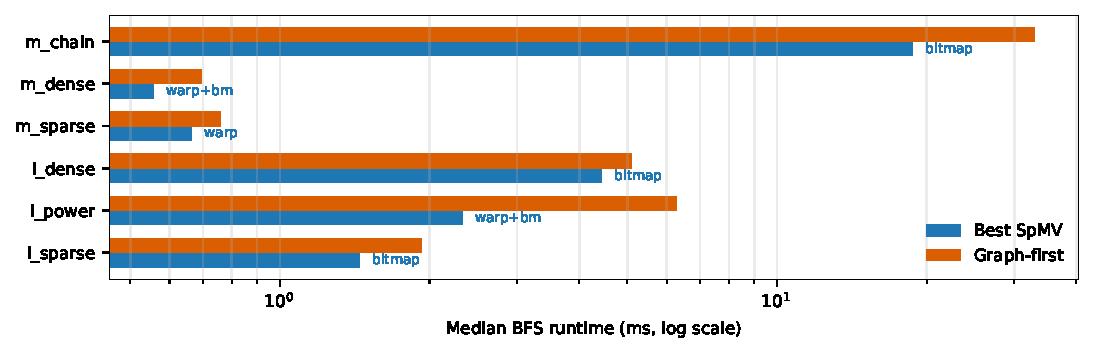
\includegraphics[width=0.78\linewidth]{figures/head_to_head_runtime.pdf}

    \vspace{-0.05em}
    \raggedright
    \textbf{Takeaways.}\ Graph-first is within $1.14\text{--}1.33\times$ on
    random sparse/dense inputs. Power-law frontiers expose queue and atomic
    update overhead; the chain graph forces 999 mostly sequential levels.
}

% =============================================================================
%  COLUMN 3 — FURTHER STUDY  (25%)
% =============================================================================
\column{0.25}

\block{9.\ Further research}{
    \raggedright
    \begin{itemize}\setlength\itemsep{8pt}
        \item \textbf{Multi-GPU (2 vs.\ 4 GPUs per node).}\ Re-run the same
              validation and timing harness on Perlmutter jobs that allocate
              two and four A100s, keeping a simple 1D CSR vertex split and
              exchanging boundary frontiers with NCCL (or MPI). The goal is an
              apples-to-apples curve: how much of the single-GPU advantage
              survives once frontier traffic and load imbalance cross NVLink,
              and whether 4-GPU runs amortize setup enough to beat 2-GPU on
              identical budgets.

        \item \textbf{Warp--bitmap fused SpMV (not emphasized on the poster).}\ The
              repo implements \texttt{warpbitmap} for linear SpMV BFS, but we
              lead with the four standalone kernels here. Next step is a focused
              study: when does fusing cooperative row scans with a bitmap
              frontier beat the best non-fused pick, how does it interact with
              push--pull scheduling, and on which graphs does the extra
              $32\times$ thread launch footprint dominate? That lines up with
              README tables once graph-first has a matching breakdown.

        \item \textbf{Harder inputs.}\ Fold in SNAP / GAP / road instances and
              compare against \textbf{cuGraph} once multi-GPU baselines exist.
    \end{itemize}
    \vspace{2.5em}
}

\block{10.\ Runtime (kernel ms)}{
    \scriptsize
    \setlength{\tabcolsep}{2.5pt}
    \raggedright
    \textbf{Linear-algebraic SpMV} (Perlmutter A100; median of 10 runs).
    Times in ms; \textbf{bold} = best per row.

    \vspace{0.25em}
    \centering
    \begin{tabular}{@{}l rr rrrrr@{}}
        \toprule
        & $\bar d$ & dep & Bsln & Wrp & Bmp & P/P & W+B \\
        \midrule
        \multicolumn{8}{@{}l}{\itshape Medium ($10^3$ vertices)} \\
        \texttt{m\_chain} & 2 & 999 & 19.55 & 19.29 & \textbf{18.73} & 32.50 & 19.22 \\
        \texttt{m\_dense} & 100 & 2 & 0.61 & 2.39 & 0.60 & 0.67 & \textbf{0.56} \\
        \texttt{m\_sparse} & 6 & 6 & 0.69 & \textbf{0.67} & 0.68 & 0.80 & 0.67 \\
        \midrule
        \multicolumn{8}{@{}l}{\itshape Large ($10^5$ vertices)} \\
        \texttt{l\_dense} & 100 & 4 & 4.92 & 5.01 & \textbf{4.44} & 4.81 & 8.10 \\
        \texttt{l\_power} & 40 & 3 & 2.83 & 8.70 & 2.47 & 4.42 & \textbf{2.33} \\
        \texttt{l\_sparse} & 10 & 7 & 1.71 & 1.81 & \textbf{1.45} & 1.81 & 1.58 \\
        \bottomrule
    \end{tabular}

    \vspace{0.55em}
    \raggedright
    \textbf{Graph-first} direction-optimizing hybrid. TD/BU counts show how
    many top-down vs.\ bottom-up kernel launches the alpha/beta heuristic chose.

    \vspace{0.2em}
    \centering
    \begin{tabular}{@{}l rr rr@{}}
        \toprule
        & $\bar d$ & dep & ms & TD/BU \\
        \midrule
        \texttt{m\_chain} & 2 & 999 & 32.92 & 1000/0 \\
        \texttt{m\_dense} & 100 & 2 & 0.70 & 1/2 \\
        \texttt{m\_sparse} & 6 & 6 & 0.76 & 4/3 \\
        \midrule
        \texttt{l\_dense} & 100 & 4 & 5.09 & 3/2 \\
        \texttt{l\_power} & 40 & 3 & 6.26 & 2/2 \\
        \texttt{l\_sparse} & 10 & 7 & 1.93 & 5/3 \\
        \bottomrule
    \end{tabular}
}

\block{11.\ References \& Code}{
    \footnotesize
    \begin{thebibliography}{9}
    \setlength\itemsep{1pt}
    \bibitem{beamer2012}
        S.\ Beamer, K.\ Asanovi\'c, D.\ Patterson.\
        \emph{Direction-Optimizing BFS.}\ SC '12.
    \bibitem{merrill2012}
        D.\ Merrill, M.\ Garland, A.\ Grimshaw.\
        \emph{Scalable GPU Graph Traversal.}\ PPoPP '12.
    \bibitem{kepner2016}
        J.\ Kepner et~al.\
        \emph{Mathematical Foundations of the GraphBLAS.}\ HPEC '16.
    \bibitem{gap}
        S.\ Beamer et~al.\
        \emph{The GAP Benchmark Suite.}\ arXiv:1508.03619, 2015.
    \bibitem{cugraph}
        NVIDIA RAPIDS.\ \emph{cuGraph: GPU graph analytics.}\
        \texttt{github.com/rapidsai/cugraph}.
    \end{thebibliography}
    \vspace{0.2em}
    \textit{Computations on NERSC \emph{Perlmutter} (NVIDIA A100,
    \texttt{sm\_80}).\ Source, build scripts, validation harness:}
    \texttt{github.com/Harshaan-Chugh/parallel-bfs}.
}

\end{columns}

\end{document}
